\section{t-критерий Стьюдента}
Давайте используем эти знания чтобы улучшить доверительный интервал $
[ \widehat{\theta} - z^{(1 - \alpha) } \cdot \widehat{\text{se}}, \ \widehat{\theta} - z^{(\alpha)} \cdot \widehat{\text{se}}]$. Как мы знаем, этот интервал выводится из предположения, что:
\begin{gather}\label{12.17}
Z = \frac{\widehat{\theta} - \theta}{\widehat{\text{se}}} \dot{\sim} \mathrm{N}(0, 1).
\end{gather}
Это справедливо при $ n \rightarrow \infty $, но для конечных выборок это приближение. Еще в $ 1908 $ году Госсет вывел лучшее приближение для случая когда $ \widehat{\theta} = \overline{x}$:
\begin{gather}\label{12.18}
Z = \frac{\widehat{\theta} - \theta}{\widehat{\text{se}}} \dot{\sim} t_{n - 1},
\end{gather}
где $t_{n - 1}$ --- распределение Стьюдента с $n - 1$ степеням свободы. 
\begin{figure}[ht]
\center{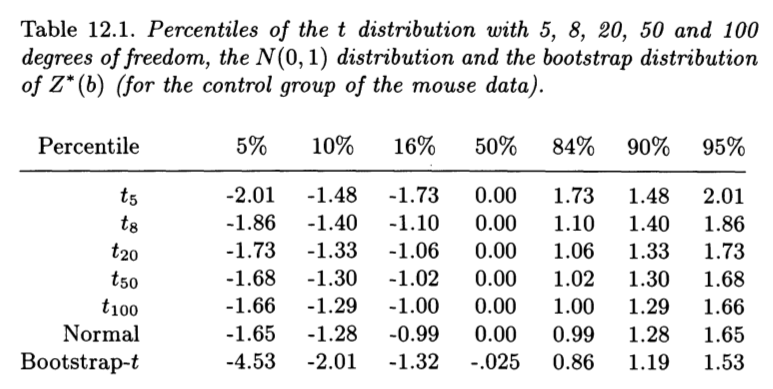
\includegraphics[width=1 \linewidth]{12/t12.2.png}}
\end{figure}
Используя это приближение, интервал равен: 
\begin{gather}\label{12.19}
[ \widehat{\theta} - t^{(1 - \alpha)}_{n-1} \cdot \widehat{\text{se}},\ \widehat{\theta} - t^{(\alpha)}_{n-1} \cdot \widehat{\text{se}}],
\end{gather}
где $t^{(\alpha)}_{n-1}$ обозначает $\alpha$ процентиль распределения Стьюдента c $n - 1$ степеням свободы. То есть, мы ищем соответствующий процентиль в $t_{n-1}$ таблице.

В таблице 12.1 показаны процентили $t_{n-1}$ распределения для разных степеней, а так же распределения $\mathrm{N} (0, 1)$. (Значения в последней строке таблицы представляют собой <<бутстреп - t процентили>>, которые будут обсуждаться ниже). Для случая когда $ \widehat{\theta} = \overline{x}$, данное приближение является точным, для нормально распределённых наблюдений, и имеет эффект расширения интервала для корректировки поскольку стандартная ошибка неизвестна. Но следует обратить внимание, что если $n \ge 20$, то процентили распределения для $t_{n}$ не сильно отличаются от процентилей для распределения $\mathrm{N}(0, 1)$. В примере с $n = 9$ использование $5\%$ и $95\%$ процентилей из таблицы для $t$ - распределения с 8 степенями свободы приводит к интервалу:
$$56.22 \pm 1.86\cdot 13.33 = (31.22,\ 81.01),$$
что немного шире чем интервала для нормального распределения $(34.29, 78.15)$. Использование $t$-распределения не регулирует доверительный интервал для учета асимметрии выборки или других ошибок, которые могут возникнуть, если $\widehat{\theta}$ не является средним по выборке. В следующем разделе описывается бутстреп - t интервал, процедура, которая эти ошибки корректирует.
